\section{Parallelized algorithms}
\label{sec:impl}

In the following implementations, we always use a similarity matrix with $1$ on its diagonal (symbols match) and $-1$ elsewhere (symbols do not match). The gap penalty is set to $p=-1$ (instead of $-2$ beforehand in the examples in \autoref{sec:needleman-wunsch}).

\subsection{On the CPU}

First, we implement the Needleman-Wunsch algorithm in Python using \tcboxverb{numpy}. This implementation serves well to deepen the understanding of the algorithm and to eliminate index errors. However, it is very slow, making it unsuitable for the whole dataset. We then translate the code to an unparallelized Rust version and confirm correct output by direct comparison with the Python implementation. To make use of all CPU cores, we \textbf{parallelize the Rust implementation} employing the \tcboxverb{rayon} library to parallelize the outer for-loop (\autoref{algstep:nested1}): for every word $A$, we consider all other words $B$ and calculate the similarity between $A$ and $B$. Since words lengths differ, the core calculation takes different times for different word pairs. Therefore, every thread appends its result to a vector that is wrapped in a \tcboxverb{Mutex} (avoid data races by mutual exclusion) and an \tcboxverb{Arc} (thread-safe reference pointer to deallocate data at the end).

Since comparing $A$ to $B$ yields the same score as the comparison of $B$ to $A$, we deal with \textit{undirected} edges and thus the adjacency matrix is symmetric. Furthermore, we are not interested in self-loops, but only in the similarity between \textit{different} words. For these two reasons, \textbf{we only consider the upper triangular part of the adjacency matrix} in \autoref{fig:traverse-schema}. To store the resulting edge weights in a binary file, we traverse the matrix in row-major order (red path): $(0,1)$, $(0,2)$, \ldots, $(0,n-1)$, $(1,2)$, \ldots, $(1,n-1), (2,3), \ldots, (n-2,n-1)$, where $n$ is the total number of words. Note that in the parallelized Rust implementation, we have to also return the indices of the words since the order in which the threads terminate is not deterministic (from point of view of the Rust code). After all threads are finished, the results are sorted according to row-major ordering to match the traversal order. When saving the edge weights in a file, we drop the indices and only store the similarity scores as 8-bit signed integers (range $[-128,127]$). This is sufficient since word lengths are typically small and match/mismatch score as well as gap penalty $p$ are likewise chosen to be small.


\subsection{On the GPU}

We implement the algorithm in the CUDA framework and deploy it on a consumer Nvidia GeForce GTX 1060 with 6GB GDDR5. We use the Driver Version 572.42 and CUDA Toolkit 12.8 inside WSL2 (Ubuntu 22.04 jammy). We consult the \tcboxverb{cudarc} Rust library, which provides Rust wrappers around the CUDA driver API as well as the NVRTC API (among others). The latter makes available a method to compile our \Cpp~kernel to \gls{ptx} code during runtime and to launch it afterwards.

Foster's methodology can help in designing parallel algorithms. The first step is to partition the problem at hand into small tasks. At the level of the adjacency matrix (\autoref{fig:traverse-schema}), such a task would be to compute the similarity score between two words $A$ and $B$ at the respective row and column. On a finer granularity, we can also refer to \autoref{fig:matrix-nuance-puissance-subcalc} and consider the calculation of one element of the score matrix. However, we realize that calculations of elements in the score matrix are highly dependent on each other since the score of a cell depends on the scores of its up, left and up-left (diagonal) neighbors (example of a \textit{stencil computation}). Additionally, words length differ, so the size of the score matrix varies. Due to the data dependencies and the varying problem size, we decide to focus on parallelizing the for-loops in the Needleman-Wunsch algorithm (lines \ref{algstep:nested1} and \ref{algstep:nested2} in \autoref{alg:needleman-wunsch}) making this a \textit{pleasingly parallel} problem, namely that of parallelizing score calculation for entries in the adjacency matrix.

The maximum number of blocks in a grid (grid size) is limited to $2^{16} - 1 = 65535$ in $y$ and $z$ direction. Starting with CUDA compute capability 3.0, the limit in the $x$ direction is raised to $2^{31} - 1 = 2,147,483,647$ blocks. Furthermore, we only consider the upper triangular part of the adjacency matrix, while a grid is always rectangular. These constraints motivate the choice of using a one-dimensional grid and spawning blocks only in the $x$ direction. Likewise, we only employ one-dimensional blocks, \ie a block is a one-dimensional array of threads. The exact number of threads we use inside a block (block dimension) is discussed later. With this configuration, we calculate (in every thread) an \textbf{index} ranging from $0$ to a number great than that of entries in the upper triangular part of the adjacency matrix:
\begin{align}
    \text{idx} = \text{blockDim.x} \cdot \text{blockIdx.x} \cdot \text{threadIdx.x}
\end{align}
This index needs to be mapped to the corresponding row and column in the adjacency matrix, such that a thread knows which words to compare. We take advantage of the row-major traversal path. Let $S_r$ be the number of elements traversed up to the end of row $r$. In \autoref{fig:traverse-schema}, this variable is drawn in blue. \autoref{fig:sum-example} provides an example to ease keeping track during following calculations.

\begin{figure}[H]
    \centering
    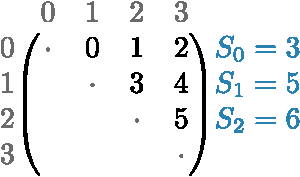
\includegraphics[width=0.5\linewidth]{assets/illustrator/sum-example.pdf}
    \caption{Example of \text{idx} (black) for $n=4$. $S_r$ is the number of elements traversed up to the end of row $r$ (blue).}
    \label{fig:sum-example}
\end{figure}

\vspace{-3em}

\begin{align}
    S_0 &= n-1, \quad S_1 = S_0 + (n-2), \quad\ldots\\
    S_r &= \sum_{k=0}^{r} (n-k-1)\\
    &= (n-1) \cdot (r+1) - \sum_{k=0}^{r} k\\
    &= (n-1) \cdot (r+1) - \frac{r \cdot (r+1)}{2}\\
    &= -\frac{1}{2}r^2 + r \left(n- \frac{3}{2}\right) + (n-1)
    \label{eq:sum-r}
\end{align}
For a given row $r$, we have $\text{idx} \in [S_{r-1}, S_r)$. We therefore require $S_{r-1} \overset{!}{=} \text{idx}$ and solve for $r$. After some algebraic manipulations, we obtain:
\begin{align}
    0 &= -\frac{1}{2} r^2 + r \underbrace{\left(n - \frac{1}{2}\right)}_z - \text{idx}\\
    \iff 0 &= r^2 + r (-2z) + 2 \cdot \text{idx}\\
    \implies r(\text{idx}) &= z - \sqrt{z^2 - 2\cdot \text{idx}}
    \label{eq:row-index}
\end{align}
We only use the negative branch of the square root since we want the row to increase with increasing index. Furthermore, we require the row index to be an integer, so we round down $\lfloor r(\text{idx}) \rfloor$ such that the row stays the same for a range of increasing indices. We can now also calculate column $c$:
\begin{align}
    c(\text{idx}) &\coloneqq r + 1 + (\text{idx} - S_{r-1})\\
    &= \frac{1}{2} r^2 + r \left(\frac{3}{2} - n\right) + (\text{idx} + 1)
\end{align}
Finally, note that $S_{n-1}$ conveniently also gives us the number of elements in the upper triangular part of the adjacency matrix, \ie the number of edges in our graph. With \eqref{eq:sum-r}, we find:
\begin{align}
    \small{\text{num edges}}
    &= S_{n-1} = \frac{1}{2} n^2 - \frac{1}{2} n
    = \frac{n(n-1)}{2}
    \label{eq:num-edges}
\end{align}

\vfill\null

TODO
